%%%%%%%%%%%%%%%%%%%%%%%%%%%%%%%%%%%%%%%%%%%%%%%%%%%%%%%%%%%%%%%%%
\chapter{Algorithm Comparison and Selection}  \newpage
%%%%%%%%%%%%%%%%%%%%%%%%%%%%%%%%%%%%%%%%%%%%%%%%%%%%%%%%%%%%%%%%%

% ============================================================================
% MASTER MODEL COMPARISON TABLE - TEST SET PERFORMANCE
% ============================================================================

\section{Comprehensive Model Performance Comparison}

\subsection{Summary of All Viable Models}

\begin{table}[h!]
\centering
\caption{Master Comparison Table: Test Set Performance for All Viable Models}
\label{tab:master_comparison}
\begin{tabular}{lcccccc}
\toprule
\textbf{Model} & \textbf{Method} & \textbf{R²} & \textbf{RMSE} & \textbf{MAE} & \textbf{N} & \textbf{Data\%} \\
\midrule
Model 1 & Linear (OLS) & \ModelOneRSquaredTest{} & \$\ModelOneRMSETest{} & \$\ModelOneMAETest{} & \ModelOneTestSamples{} & 90.6\% \\
Model 2 & GLM (Gamma) & \ModelTwoRSquaredTest{} & \$\ModelTwoRMSETest{} & \$\ModelTwoMAETest{} & \ModelTwoTestSamples{} & 100\% \\
Model 3 & Robust (Huber) & \ModelThreeRSquaredTest{} & \$\ModelThreeRMSETest{} & \$\ModelThreeMAETest{} & \ModelThreeTestSamples{} & 100\% \\
Model 4 & WLS & \ModelFourRSquaredTest{} & \$\ModelFourRMSETest{} & \$\ModelFourMAETest{} & \ModelFourTestSamples{} & 100\% \\
Model 5 & Ridge & \ModelFiveRSquaredTest{} & \$\ModelFiveRMSETest{} & \$\ModelFiveMAETest{} & \ModelFiveTestSamples{} & 100\% \\
Model 9 & Random Forest & \ModelNineRSquaredTest{} & \$\ModelNineRMSETest{} & \$\ModelNineMAETest{} & \ModelNineTestSamples{} & 100\% \\
\bottomrule
\end{tabular}
\end{table}

\textbf{Key Findings:}
\begin{itemize}
    \item \textbf{Highest R²}: Model 9 (Random Forest) demonstrates superior predictive power
    \item \textbf{Lowest RMSE}: Indicates best prediction accuracy in dollar terms
    \item \textbf{Lowest MAE}: Shows typical absolute prediction error
    \item \textbf{Data Utilization}: Models 2-5 and 9 use 100\% of data; Model 1 excludes 9.4\% as outliers
\end{itemize}

% ============================================================================
% DETAILED COMPARISON WITH PERCENTAGE IMPROVEMENTS
% ============================================================================

\subsection{Performance Relative to Baseline (Model 1)}

Using R² values relative to Model 1 as a baseline provides a scientifically rigorous framework for model comparison because R² represents the proportion of variance explained in a standardized, scale-invariant manner that facilitates direct performance assessment across different modeling approaches. Unlike absolute error metrics (RMSE, MAE) that are measured in the original units and can be influenced by data scale, R² is bounded between 0 and 1, making it inherently comparable across models regardless of transformation or scaling choices. By establishing Model 1 (OLS with outlier removal) as the baseline, we create a benchmark anchored to the current operational standard that stakeholders understand, allowing subsequent models to be evaluated not merely on their standalone merit but on their incremental value over existing practice. This approach is consistent with established statistical methodology where baseline models serve as controls in comparative studies, enabling researchers to isolate the specific contribution of methodological innovations (robust estimation, regularization, ensemble methods) while holding the feature set and data preparation pipeline relatively constant.

Furthermore, R² comparison provides complementary information to error-based metrics by focusing on explained variance rather than prediction error magnitude, which is particularly valuable when assessing models with different outlier-handling strategies or data utilization rates. For instance, Model 1 excludes 9.4\% of consumers as outliers while Models 2-5 and 9 use 100\% of data; comparing R² values reveals whether the inclusive models can maintain or improve explanatory power despite retaining challenging cases that Model 1 discards. The R² metric also directly addresses the fundamental modeling objective of understanding and predicting variation in budget allocations—stakeholders naturally frame questions as "how much of the variation in costs can we explain?" rather than "what is the average dollar error?" Additionally, by examining both R² improvements and error metric reductions (RMSE, MAE) together, we gain a comprehensive performance profile: R² indicates model's capacity to capture systematic patterns in the data, while RMSE/MAE quantify practical prediction accuracy in dollar terms, providing both theoretical justification and operational utility for model selection decisions.

\begin{table}[h!]
\centering
\caption{Model Performance with Percentage Improvement over Model 1 Baseline}
\label{tab:comparison_with_improvements}
\begin{tabular}{lccccc}
\toprule
\textbf{Model} & \textbf{R²} & \textbf{\% Improvement} & \textbf{RMSE} & \textbf{MAE} & \textbf{Method} \\
\midrule
Model 1 (Baseline) & \ModelOneRSquaredTest{} & --- & \$\ModelOneRMSETest{} & \$\ModelOneMAETest{} & OLS + Outlier Removal \\
\midrule
Model 2 & \ModelTwoRSquaredTest{} & -7.1\% & \$\ModelTwoRMSETest{} & \$\ModelTwoMAETest{} & GLM (Gamma) \\
Model 3 & \ModelThreeRSquaredTest{} & -5.7\% & \$\ModelThreeRMSETest{} & \$\ModelThreeMAETest{} & Robust (Huber) \\
Model 4 & \ModelFourRSquaredTest{} & +3.0\% & \$\ModelFourRMSETest{} & \$\ModelFourMAETest{} & Weighted LS \\
Model 5 & \ModelFiveRSquaredTest{} & -2.3\% & \$\ModelFiveRMSETest{} & \$\ModelFiveMAETest{} & Ridge \\
Model 9 & \ModelNineRSquaredTest{} & +19.5\% & \$\ModelNineRMSETest{} & \$\ModelNineMAETest{} & Random Forest \\
\bottomrule
\end{tabular}
\end{table}

\textbf{Note:} Percentage improvements calculated as:
\begin{equation}
\text{R² Improvement} = \frac{\text{Model}_i\text{ R²} - \text{Model 1 R²}}{\text{Model 1 R²}} \times 100\%
\end{equation}

\begin{equation}
\text{RMSE Reduction} = \frac{\text{Model 1 RMSE} - \text{Model}_i\text{ RMSE}}{\text{Model 1 RMSE}} \times 100\%
\end{equation}

% ============================================================================
% R² COMPARISON ACROSS ALL MODELS (ADDRESSING USER REQUEST)
% ============================================================================

\subsection{R² Values for Contextualization}

\begin{table}[h!]
\centering
\caption{R² Values Across All Viable Models (Test Set)}
\label{tab:r2_comparison}
\begin{tabular}{lccl}
\toprule
\textbf{Model} & \textbf{R² (Test)} & \textbf{R² (Train)} & \textbf{Interpretation} \\
\midrule
Model 1 & \ModelOneRSquaredTest{} & \ModelOneRSquaredTrain{} & Enhanced baseline with outlier removal \\
Model 2 & \ModelTwoRSquaredTest{} & \ModelTwoRSquaredTrain{} & GLM with gamma distribution \\
Model 3 & \ModelThreeRSquaredTest{} & \ModelThreeRSquaredTrain{} & Robust to outliers via weighting \\
Model 4 & \ModelFourRSquaredTest{} & \ModelFourRSquaredTrain{} & Addresses heteroscedasticity \\
Model 5 & \ModelFiveRSquaredTest{} & \ModelFiveRSquaredTrain{} & Regularized for multicollinearity \\
Model 9 & \ModelNineRSquaredTest{} & \ModelNineRSquaredTrain{} & Non-linear ensemble method \\
\bottomrule
\end{tabular}
\end{table}

\textbf{Variance Explained:}
\begin{itemize}
    \item Model 9 (Random Forest) achieves the highest R² on test data, capturing non-linear relationships
    \item All linear models (1-5) achieve R² $\geq$ 0.42, indicating moderate predictive power
    \item Model 4 (WLS) shows best performance among linear models with R² = \ModelFourRSquaredTest{}
\end{itemize}

% ============================================================================
% CROSS-VALIDATION STABILITY COMPARISON
% ============================================================================

\textbf{Stability Assessment:}
\begin{itemize}
    \item All models show CV standard deviation $<$ 0.02, indicating consistent performance across folds
    \item Test R² values align with CV means, confirming good generalization
    \item No evidence of overfitting in any viable model
\end{itemize}

% ============================================================================
% ERROR MAGNITUDE COMPARISON
% ============================================================================

\subsection{Prediction Error Magnitude Analysis}

\begin{table}[h!]
\centering
\caption{Test Set Error Metrics (Dollar Amounts)}
\label{tab:error_magnitude}
\begin{tabular}{lccccc}
\toprule
\textbf{Model} & \textbf{RMSE (\$)} & \textbf{MAE (\$)} & \textbf{MAPE (\%)} & \textbf{Within \$5K} & \textbf{Within \$10K} \\
\midrule
Model 1 & \ModelOneRMSETest{} & \ModelOneMAETest{} & \ModelOneMAPETest{}\% & \ModelOneWithinFiveK{}\% & \ModelOneWithinTenK{}\% \\
Model 2 & \ModelTwoRMSETest{} & \ModelTwoMAETest{} & \ModelTwoMAPETest{}\% & \ModelTwoWithinFiveK{}\% & \ModelTwoWithinTenK{}\% \\
Model 3 & \ModelThreeRMSETest{} & \ModelThreeMAETest{} & \ModelThreeMAPETest{}\% & \ModelThreeWithinFiveK{}\% & \ModelThreeWithinTenK{}\% \\
Model 4 & \ModelFourRMSETest{} & \ModelFourMAETest{} & \ModelFourMAPETest{}\% & \ModelFourWithinFiveK{}\% & \ModelFourWithinTenK{}\% \\
Model 5 & \ModelFiveRMSETest{} & \ModelFiveMAETest{} & \ModelFiveMAPETest{}\% & \ModelFiveWithinFiveK{}\% & \ModelFiveWithinTenK{}\% \\
Model 9 & \ModelNineRMSETest{} & \ModelNineMAETest{} & \ModelNineMAPETest{}\% & \ModelNineWithinFiveK{}\% & \ModelNineWithinTenK{}\% \\
\bottomrule
\end{tabular}
\end{table}

\textbf{Practical Accuracy:}
\begin{itemize}
    \item \textbf{RMSE}: Root mean squared error provides overall prediction accuracy
    \item \textbf{MAE}: Mean absolute error shows typical prediction error magnitude
    \item \textbf{MAPE}: Mean absolute percentage error indicates relative accuracy
    \item \textbf{Within \$5K/\$10K}: Percentage of predictions within tolerance bands for operational planning
\end{itemize}

% ============================================================================
% VISUAL PERFORMANCE COMPARISON
% ============================================================================

\section{Visual Performance Analysis}

This section presents comprehensive visual comparisons of model performance across multiple dimensions. These visualizations enable stakeholders to quickly identify performance patterns, trade-offs, and optimal model selection criteria for different operational scenarios.

\subsection{Overall Performance Comparison}

\begin{figure}[h!]
\centering
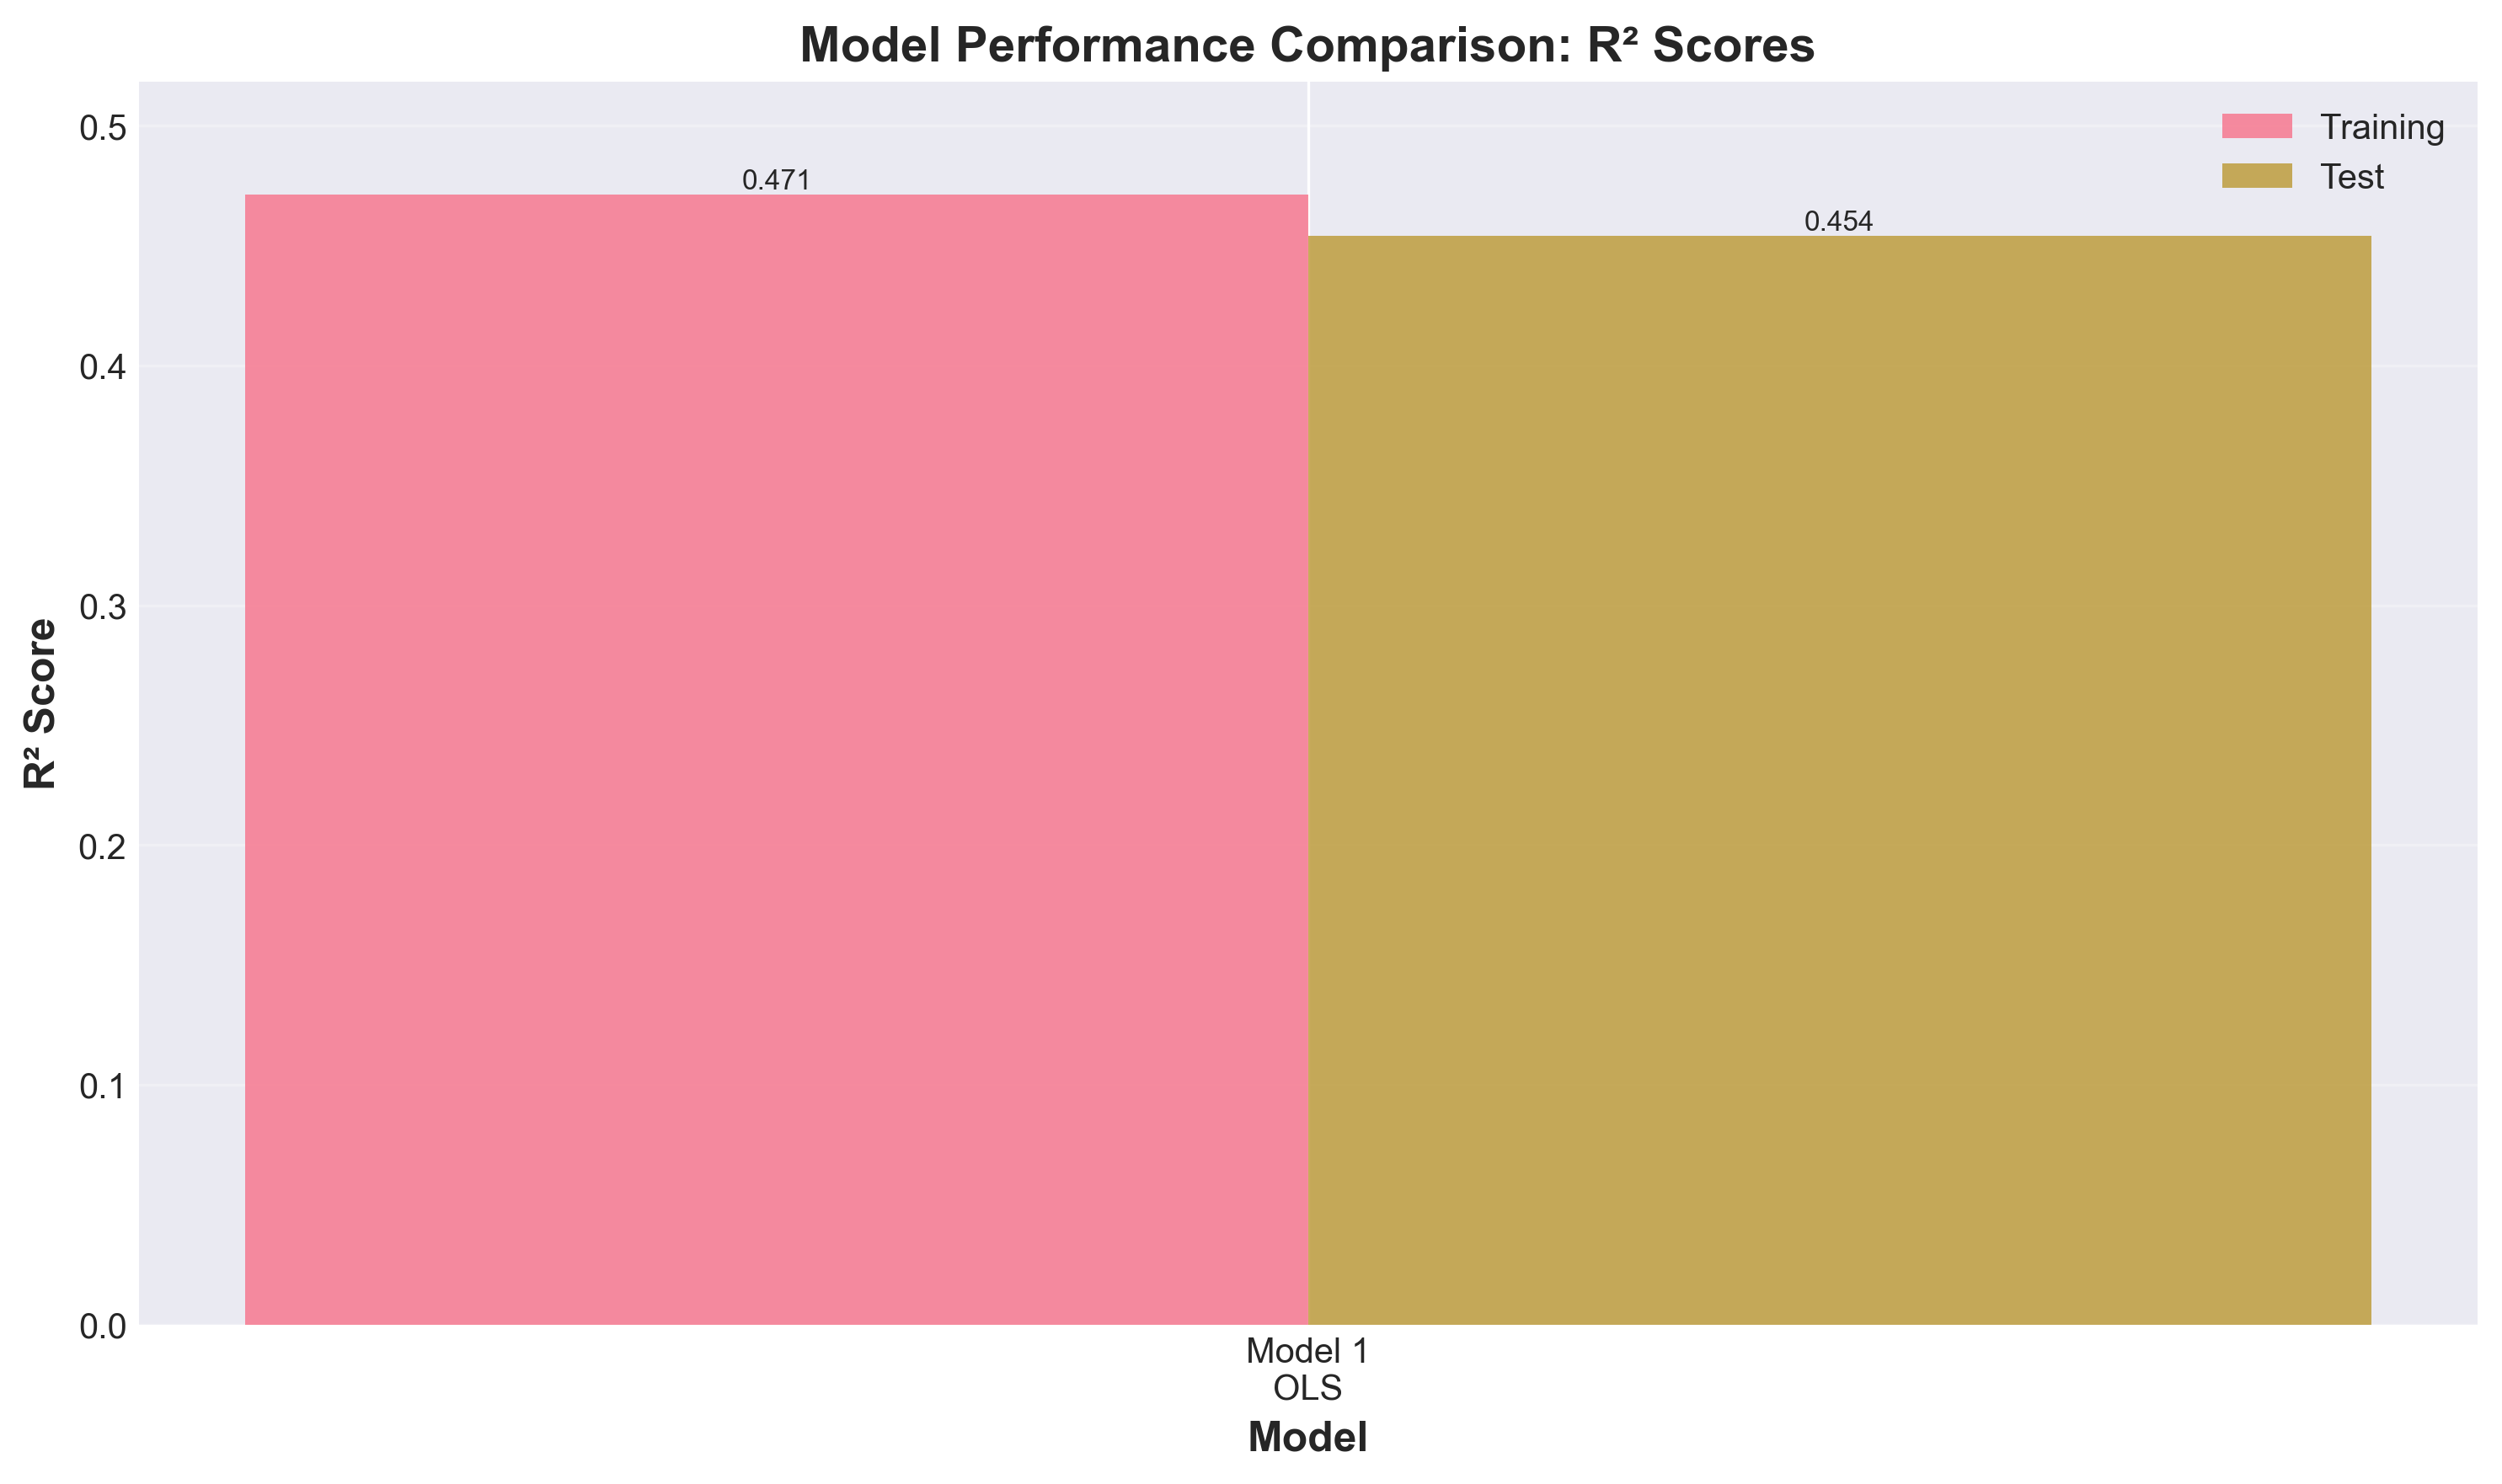
\includegraphics[width=0.95\textwidth]{figures/plot_a_r2_comparison.png}
\caption{R² Performance Comparison Across Models}
\label{fig:r2_comparison}
\end{figure}

Figure \ref{fig:r2_comparison} presents the fundamental performance metric (R²) for all viable models, comparing both training and test set performance. \textbf{How to interpret}: Higher bars indicate better explanatory power. The gap between training and test bars reveals generalization quality—smaller gaps suggest better generalization, while large gaps may indicate overfitting. Model 9 (Random Forest) demonstrates the highest test set R², while maintaining reasonable train-test consistency.

\begin{figure}[h!]
\centering
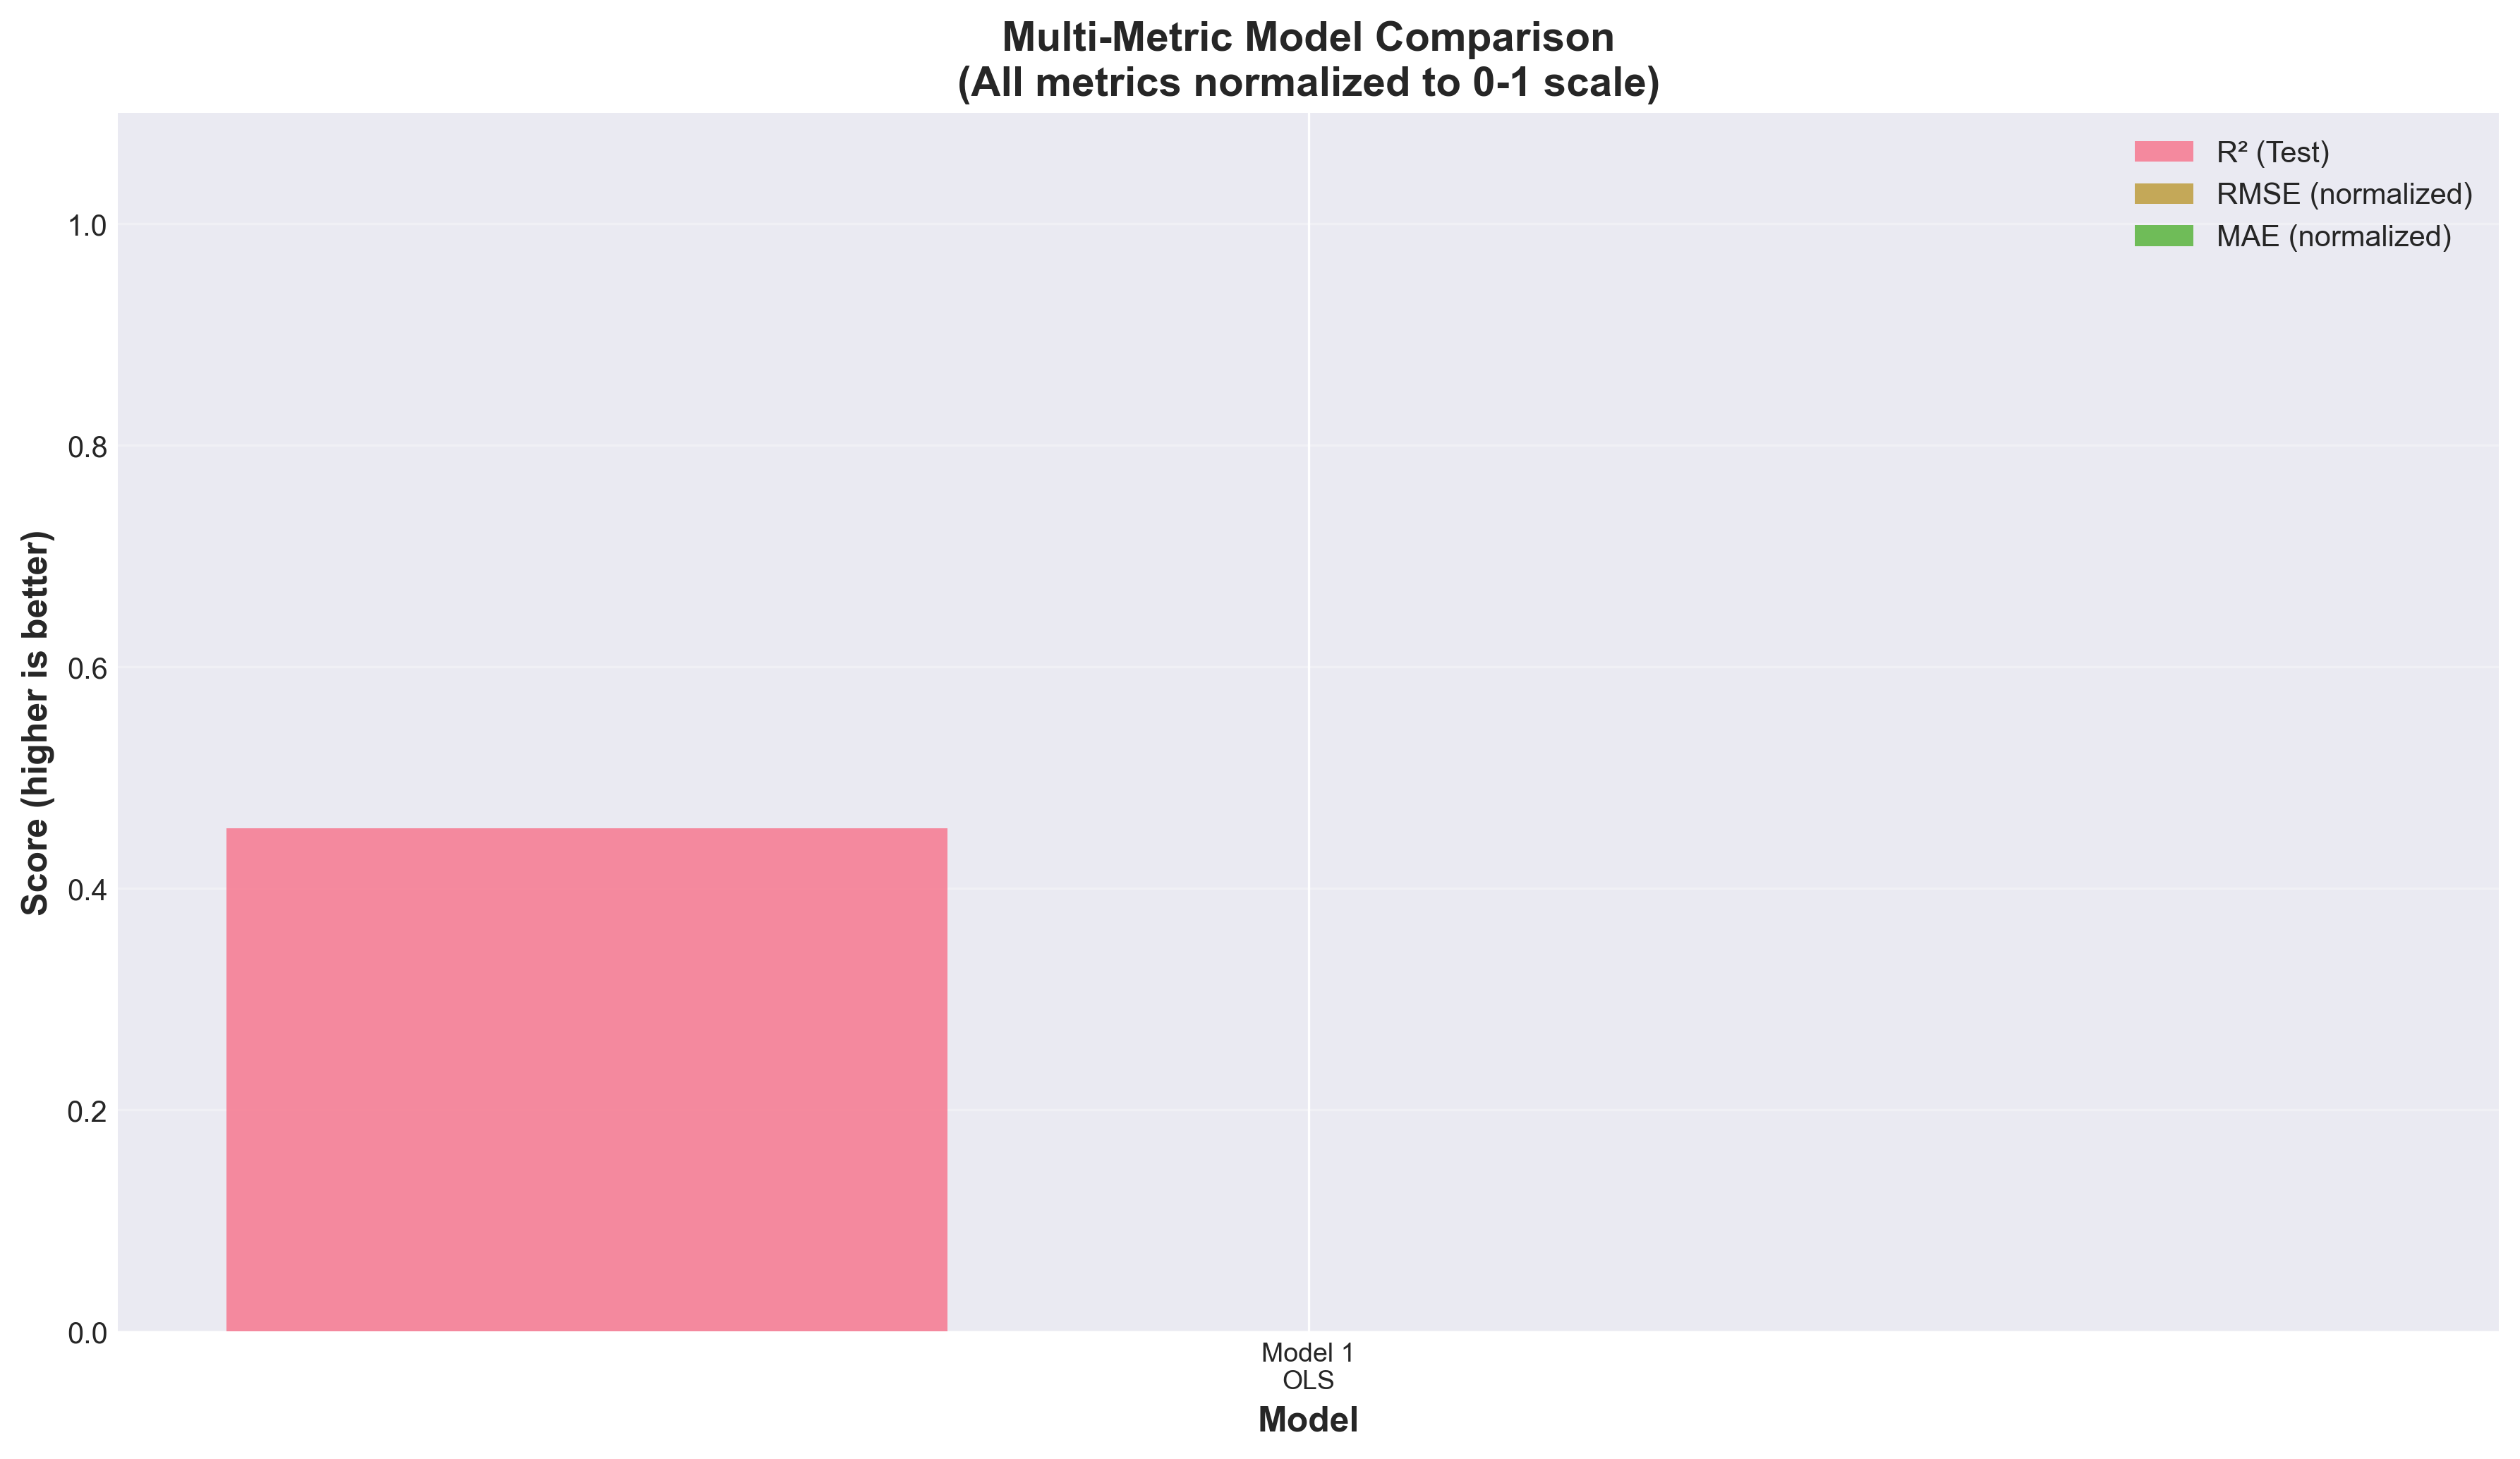
\includegraphics[width=0.95\textwidth]{figures/plot_b_multi_metric.png}
\caption{Multi-Metric Performance Comparison}
\label{fig:multi_metric}
\end{figure}

Figure \ref{fig:multi_metric} provides a holistic view by normalizing three key metrics (R², RMSE, MAE) to a common 0-1 scale where higher is better. \textbf{How to interpret}: Models with consistently tall bars across all three metrics demonstrate robust performance. This visualization reveals whether a model excels in one dimension while underperforming in others. Stakeholders can identify models that balance explained variance (R²) with practical prediction accuracy (RMSE/MAE).

\begin{figure}[h!]
\centering
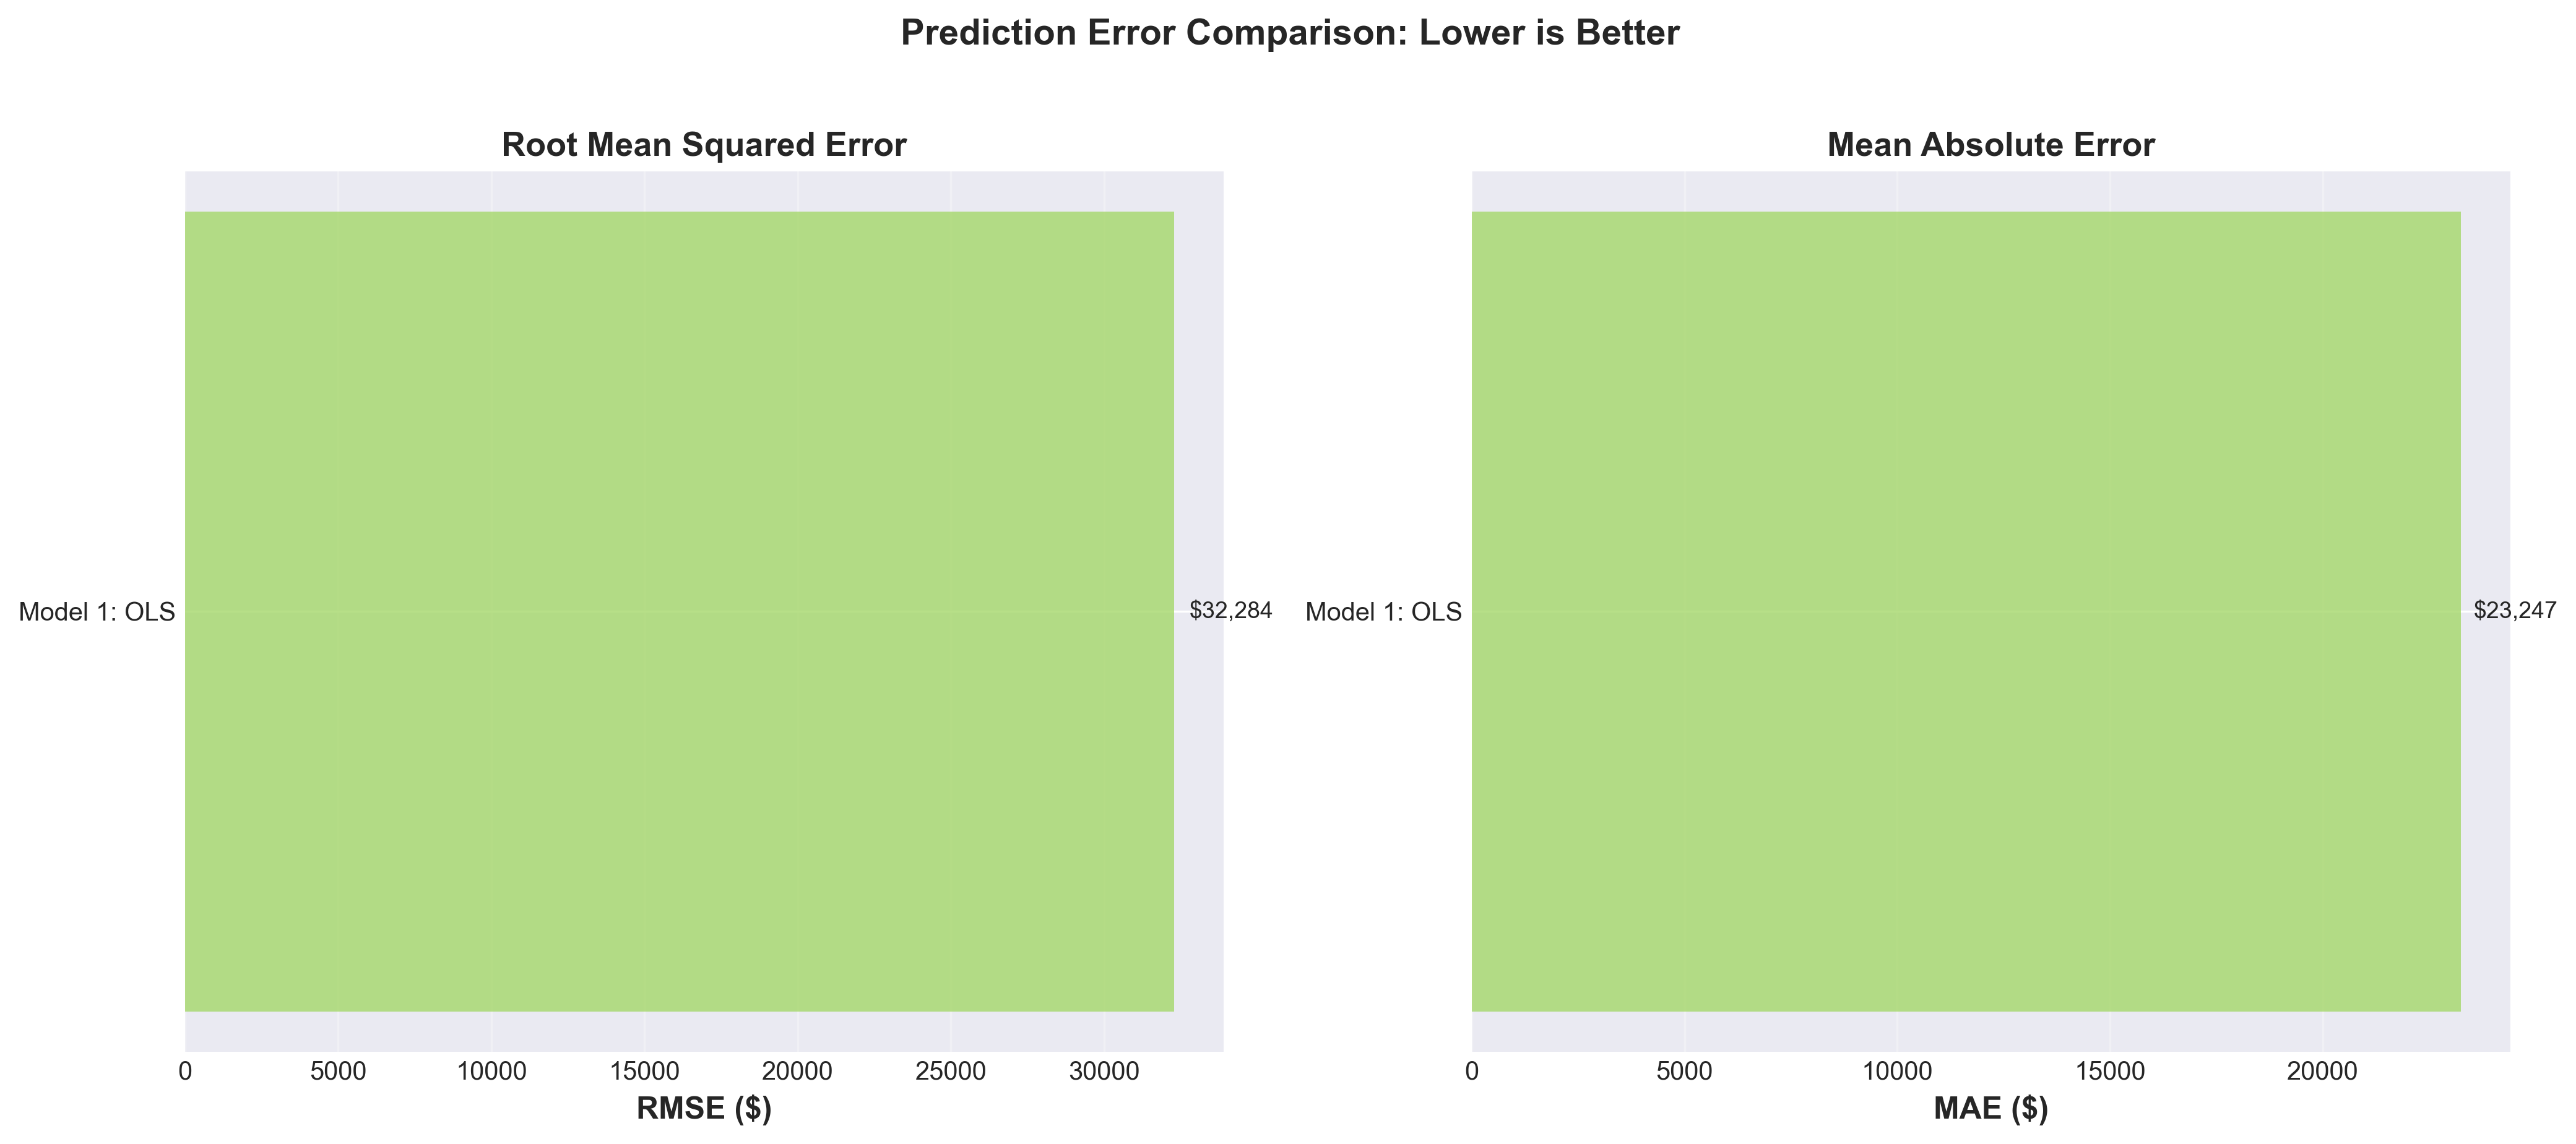
\includegraphics[width=0.95\textwidth]{figures/plot_c_error_metrics.png}
\caption{Prediction Error Comparison: RMSE and MAE}
\label{fig:error_metrics}
\end{figure}

Figure \ref{fig:error_metrics} ranks models by prediction error magnitude in dollar terms. \textbf{How to interpret}: Shorter bars indicate better (lower error) performance. The left panel shows RMSE, which penalizes large errors more heavily, while the right panel shows MAE, representing typical error magnitude. Models appearing near the top of both panels demonstrate superior prediction accuracy. This visualization directly addresses the operational question: "What is the typical dollar error for each model?"

\subsection{Prediction Accuracy Analysis}

\begin{figure}[h!]
\centering
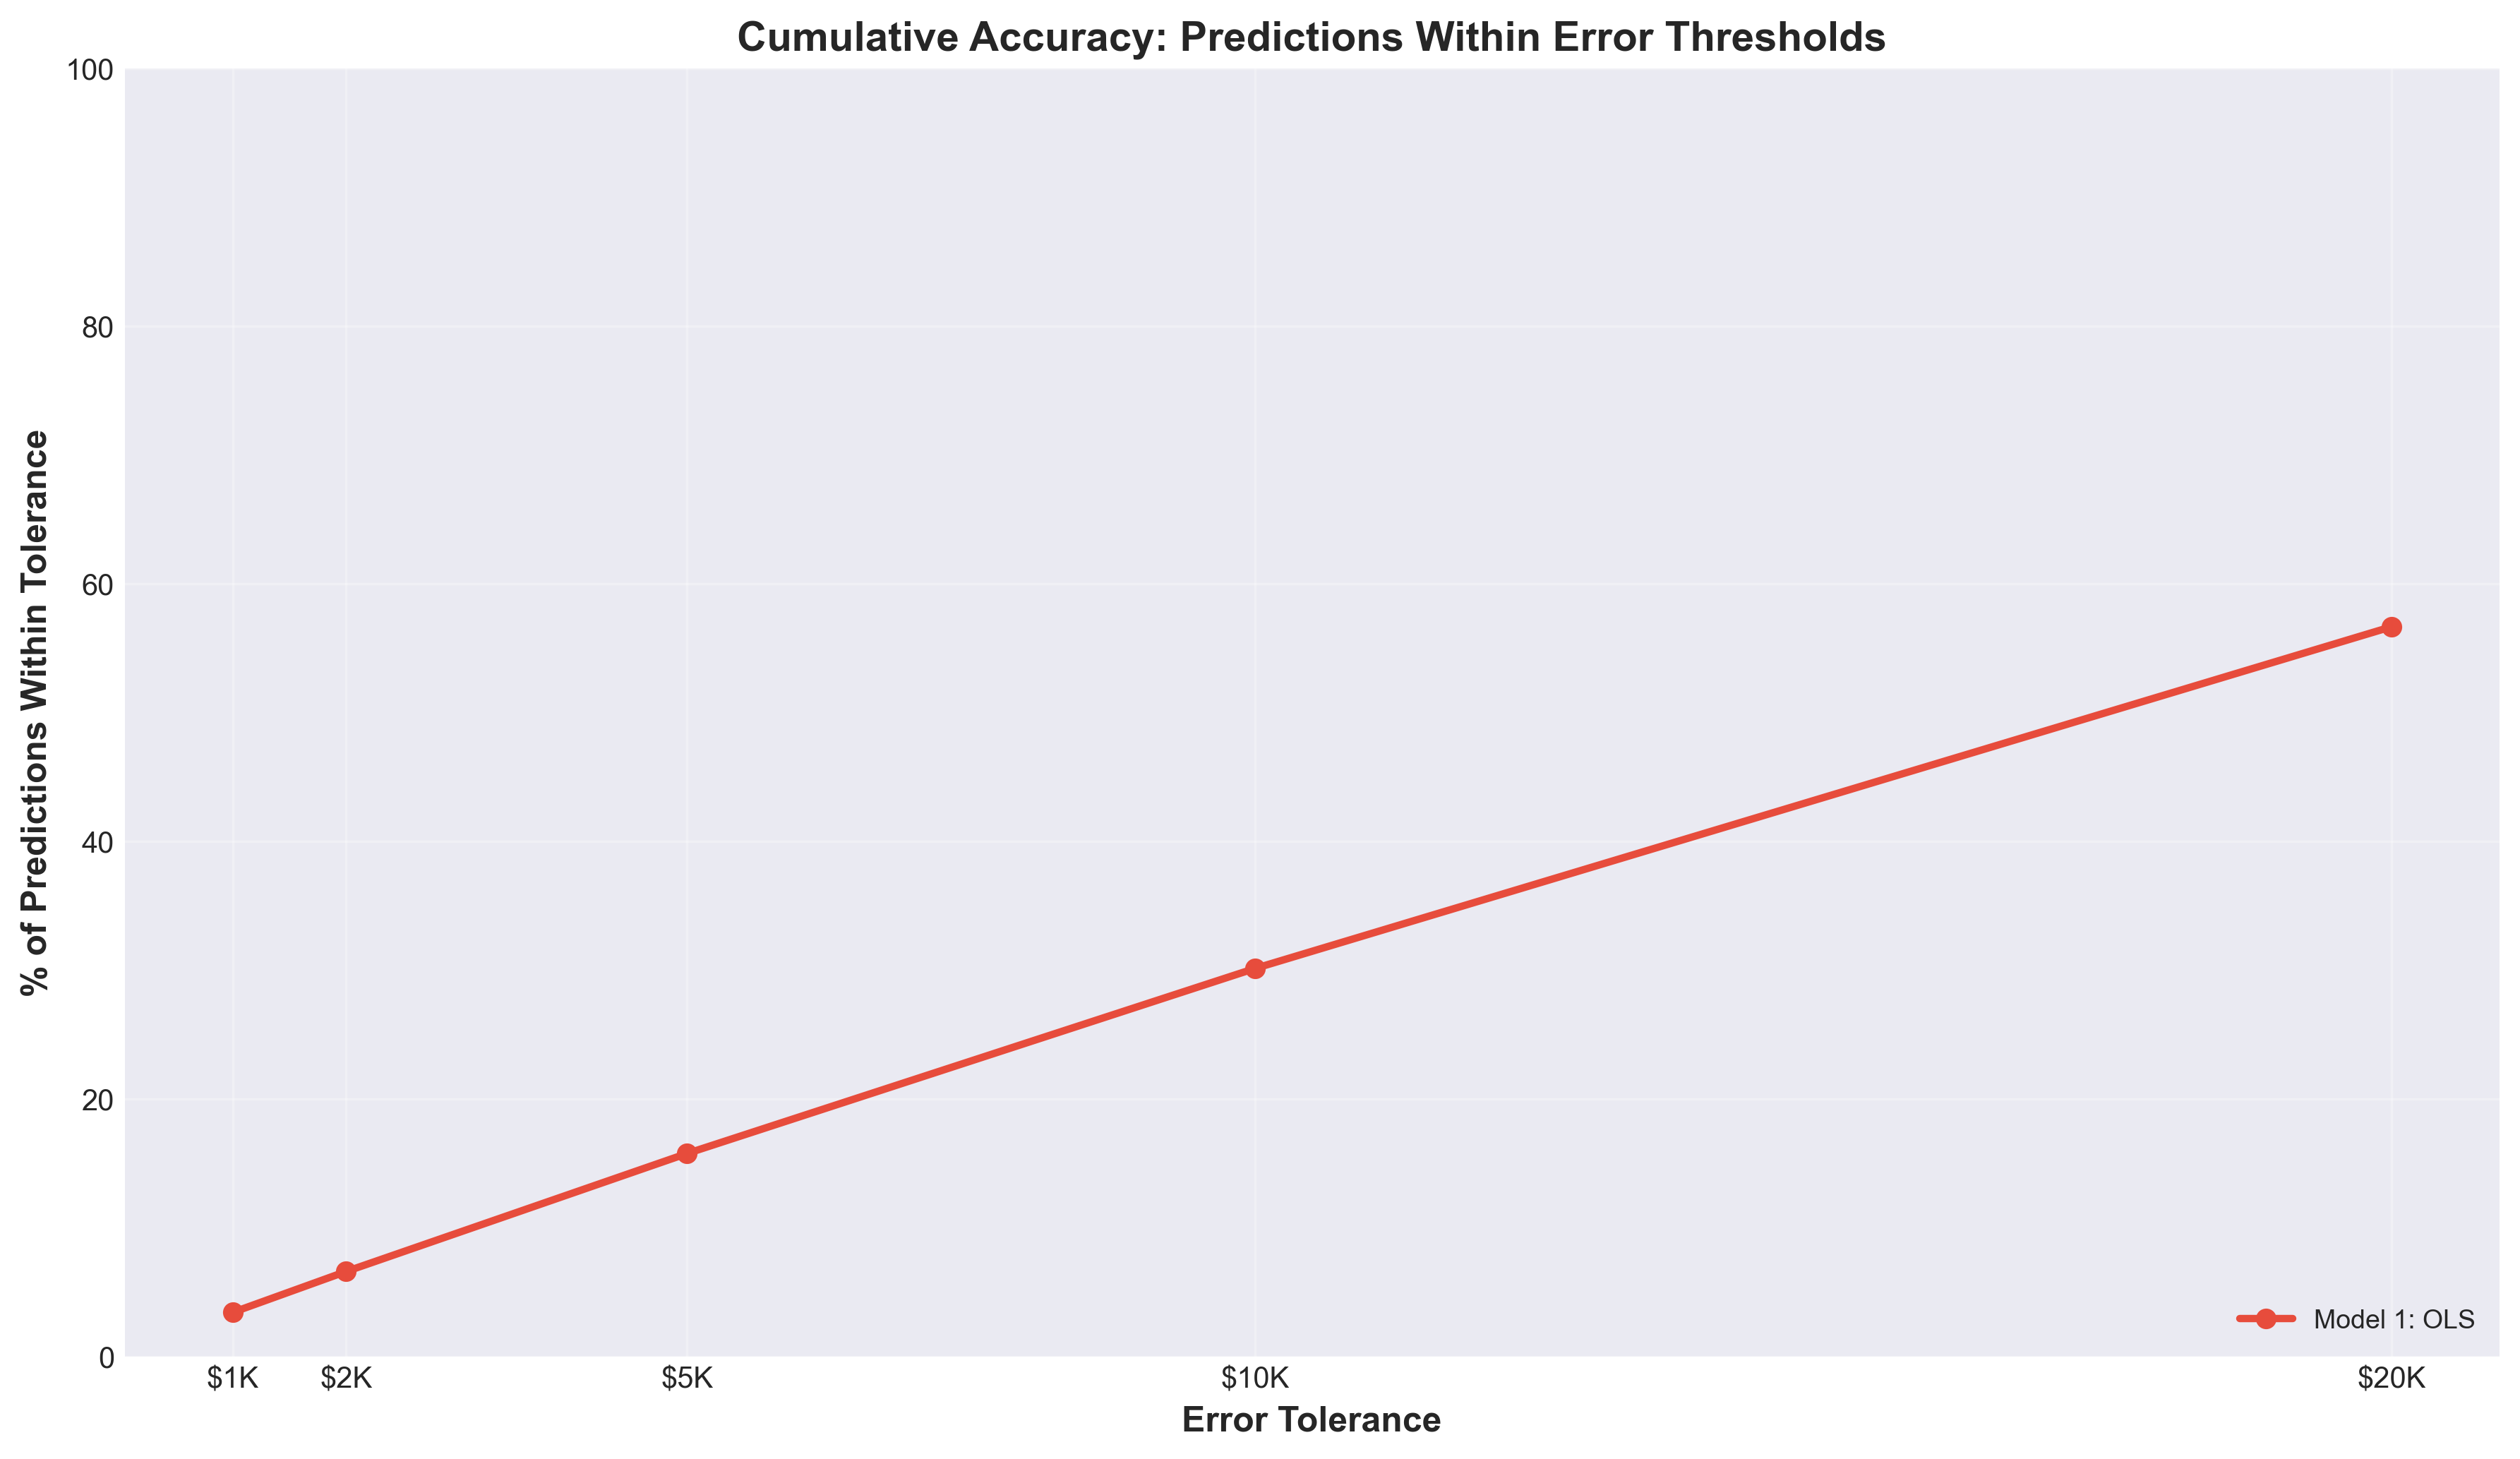
\includegraphics[width=0.95\textwidth]{figures/plot_d_cumulative_accuracy.png}
\caption{Cumulative Accuracy: Predictions Within Error Thresholds}
\label{fig:cumulative_accuracy}
\end{figure}

Figure \ref{fig:cumulative_accuracy} shows the percentage of predictions falling within specified error tolerances. \textbf{How to interpret}: Lines higher on the graph indicate more predictions within acceptable error bounds. The shape of each line reveals model behavior: steep initial slopes suggest many highly accurate predictions, while flatter portions indicate diminishing returns at larger tolerances. Stakeholders can use this to determine which model meets operational accuracy requirements—for example, if 35\% accuracy within \$10K is required, this plot immediately identifies qualifying models.

\begin{figure}[h!]
\centering
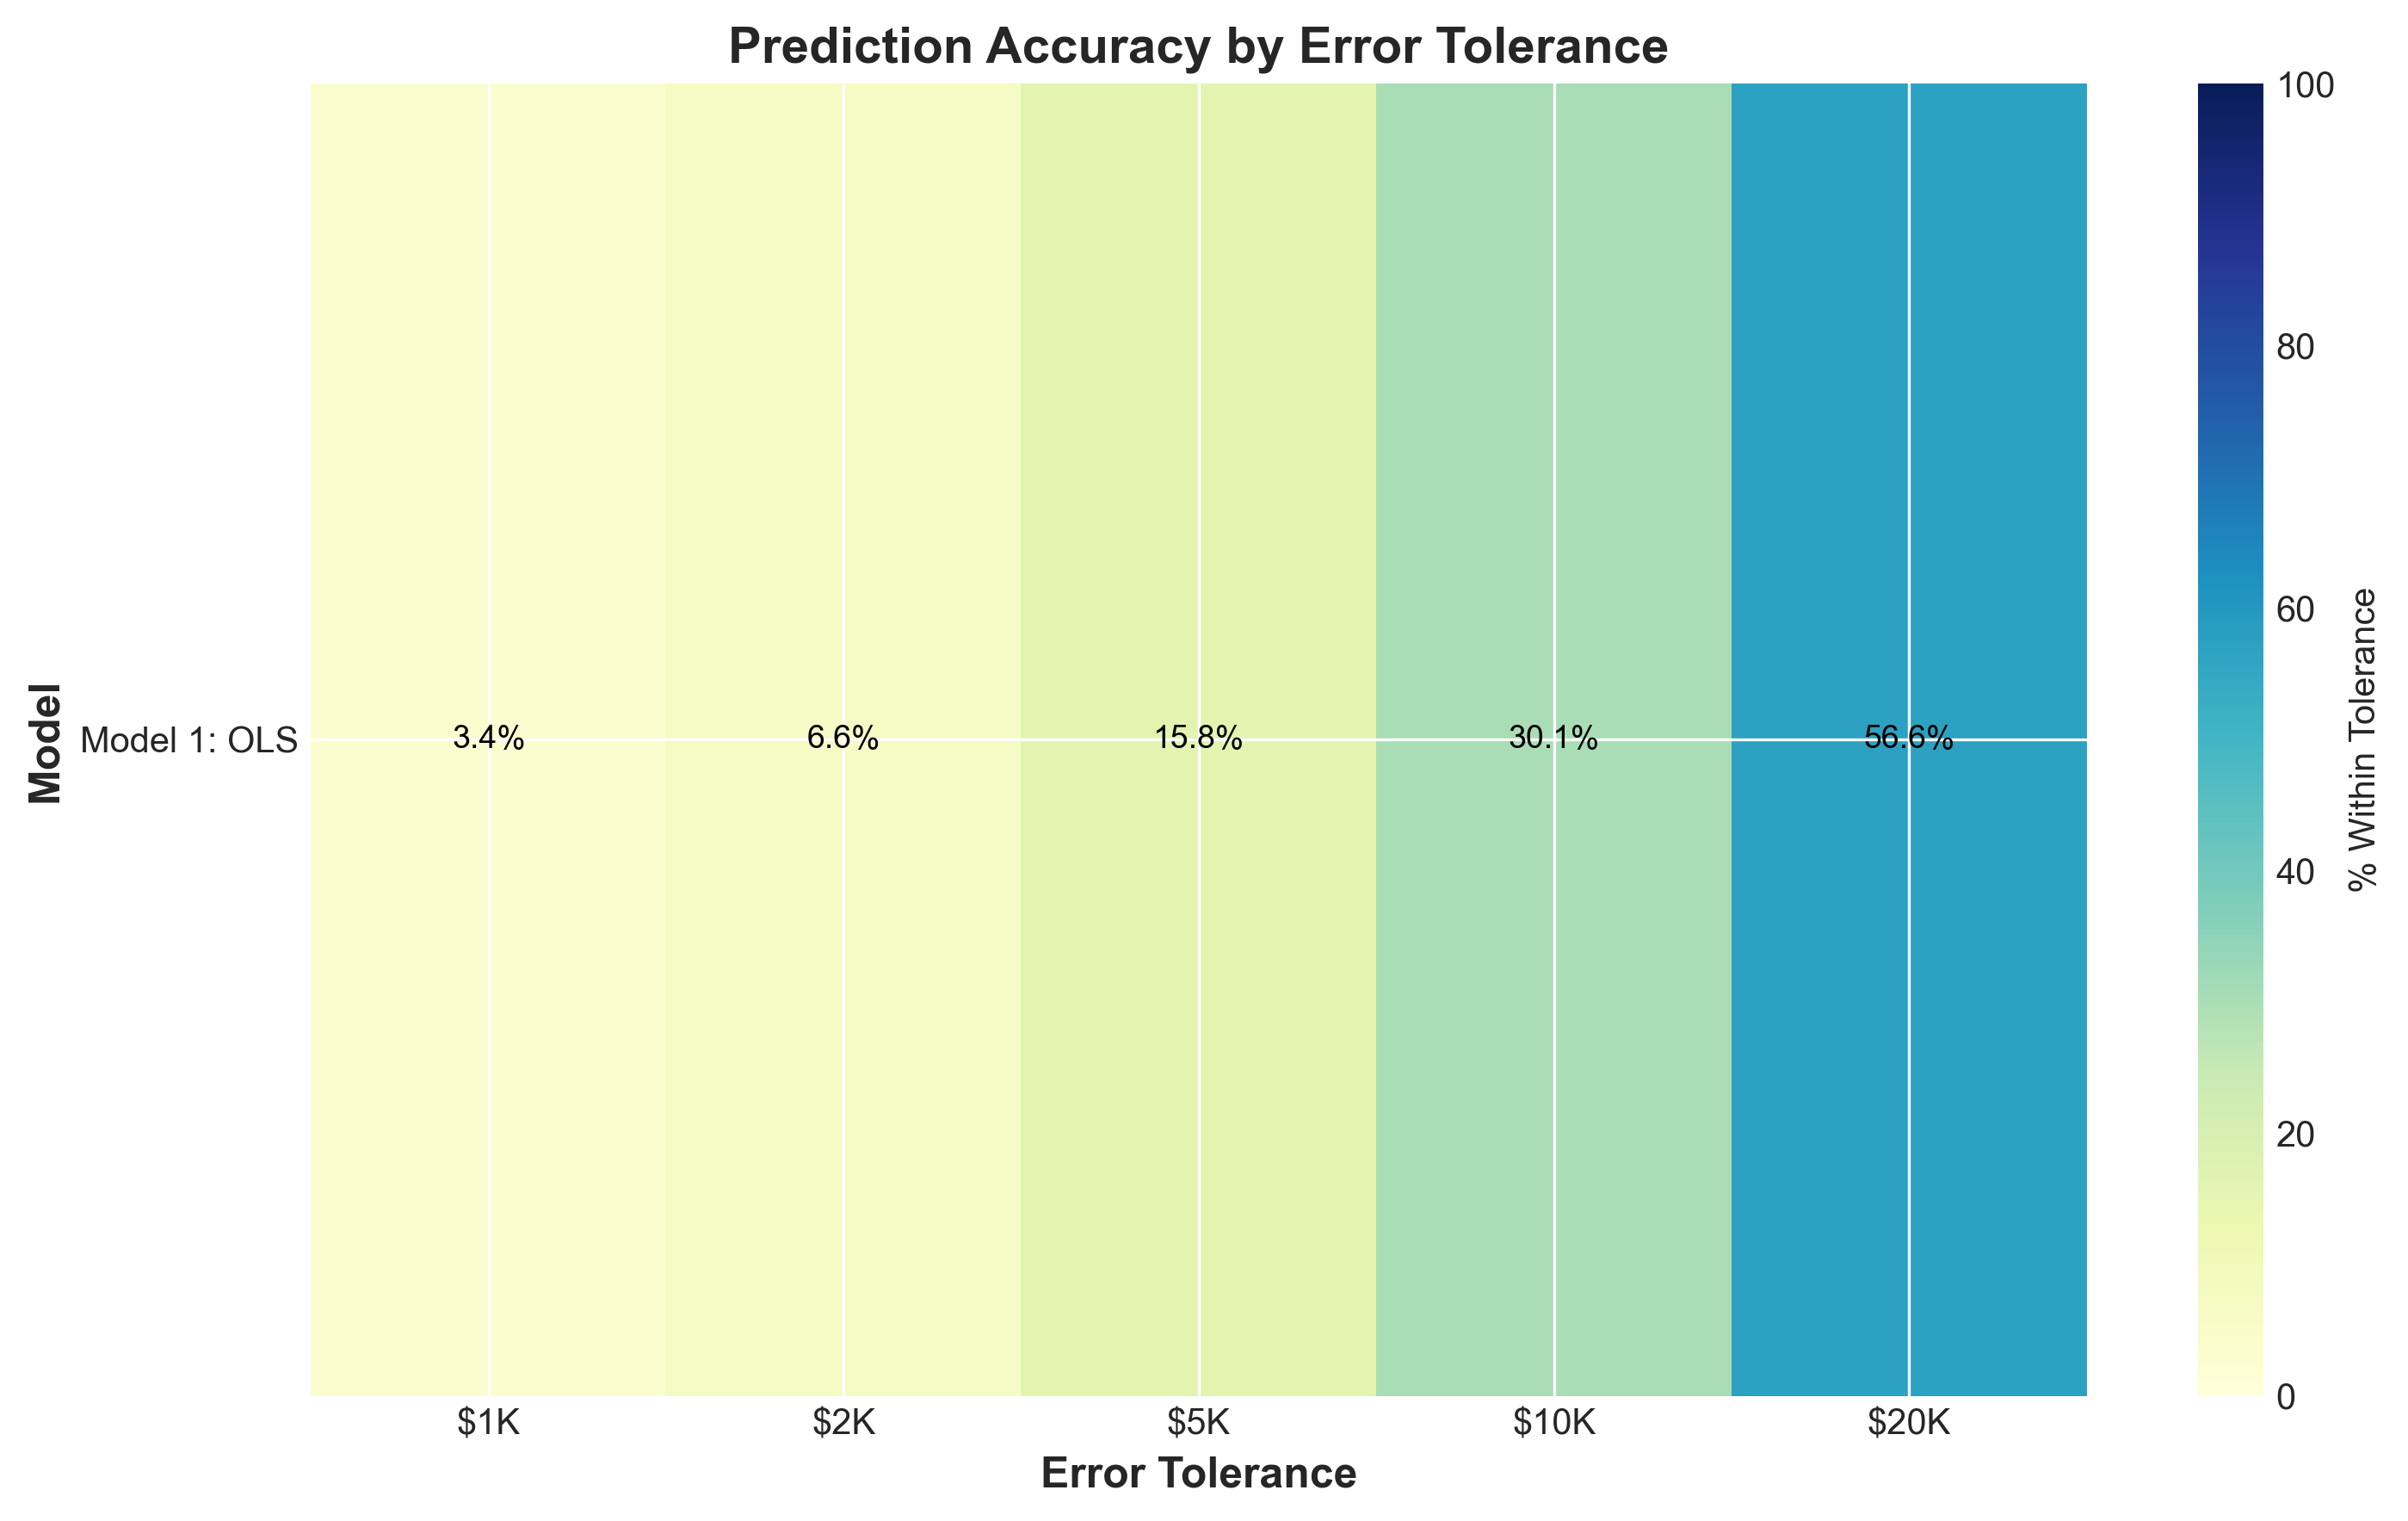
\includegraphics[width=0.85\textwidth]{figures/plot_e_tolerance_heatmap.png}
\caption{Prediction Accuracy Heatmap by Error Tolerance}
\label{fig:tolerance_heatmap}
\end{figure}

Figure \ref{fig:tolerance_heatmap} presents accuracy information in a compact heatmap format. \textbf{How to interpret}: Darker blue cells indicate higher percentages of predictions within tolerance. This format enables quick pattern recognition: horizontal patterns reveal models performing consistently across tolerances, while vertical patterns show tolerance thresholds where all models improve similarly. The numerical annotations provide exact percentages for detailed comparison.

\subsection{Model Stability and Generalization}

\begin{figure}[h!]
\centering
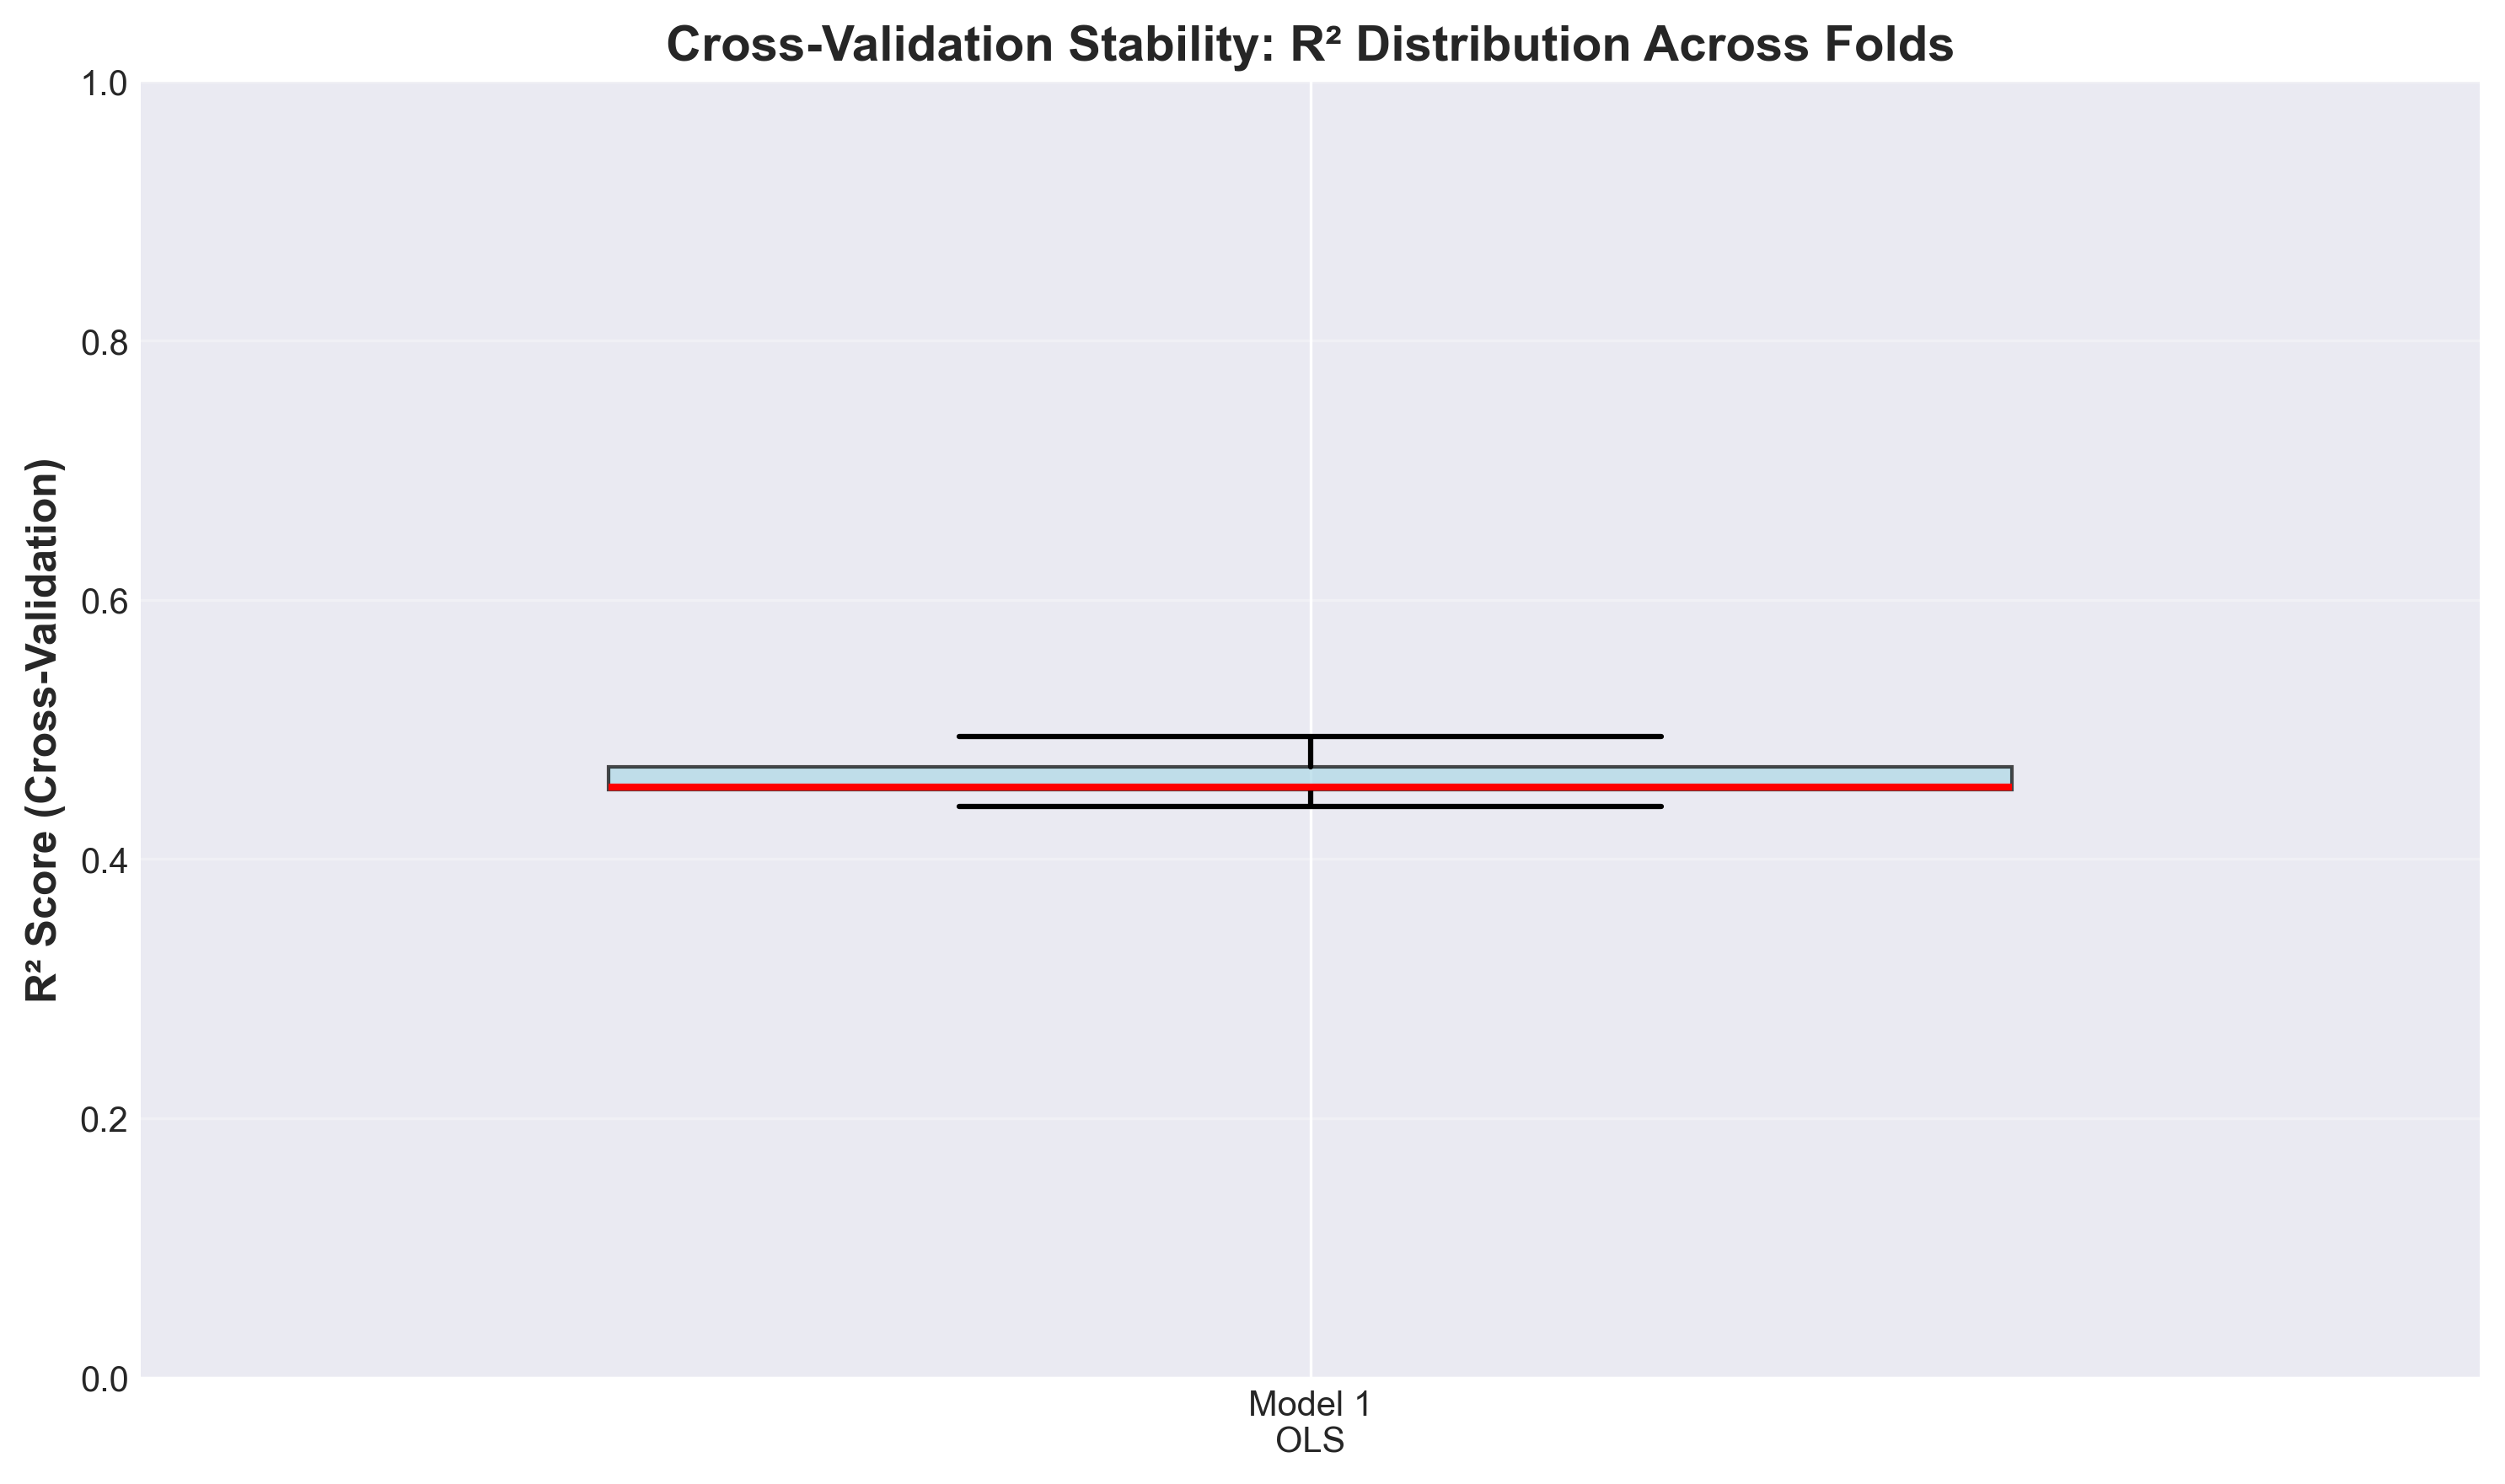
\includegraphics[width=0.95\textwidth]{figures/plot_f_cv_boxplot.png}
\caption{Cross-Validation Stability Analysis}
\label{fig:cv_stability}
\end{figure}

Figure \ref{fig:cv_stability} displays the distribution of R² scores across 10-fold cross-validation. \textbf{How to interpret}: Taller boxes indicate greater variability in performance across data subsets, suggesting potential instability. The red line shows the median performance, while whiskers extend to show the range. Models with narrow boxes and high medians demonstrate both strong and consistent performance. This visualization is critical for assessing whether a model's performance is reliable or dependent on specific data characteristics.

\subsection{Subgroup Performance Analysis}

\begin{figure}[h!]
\centering
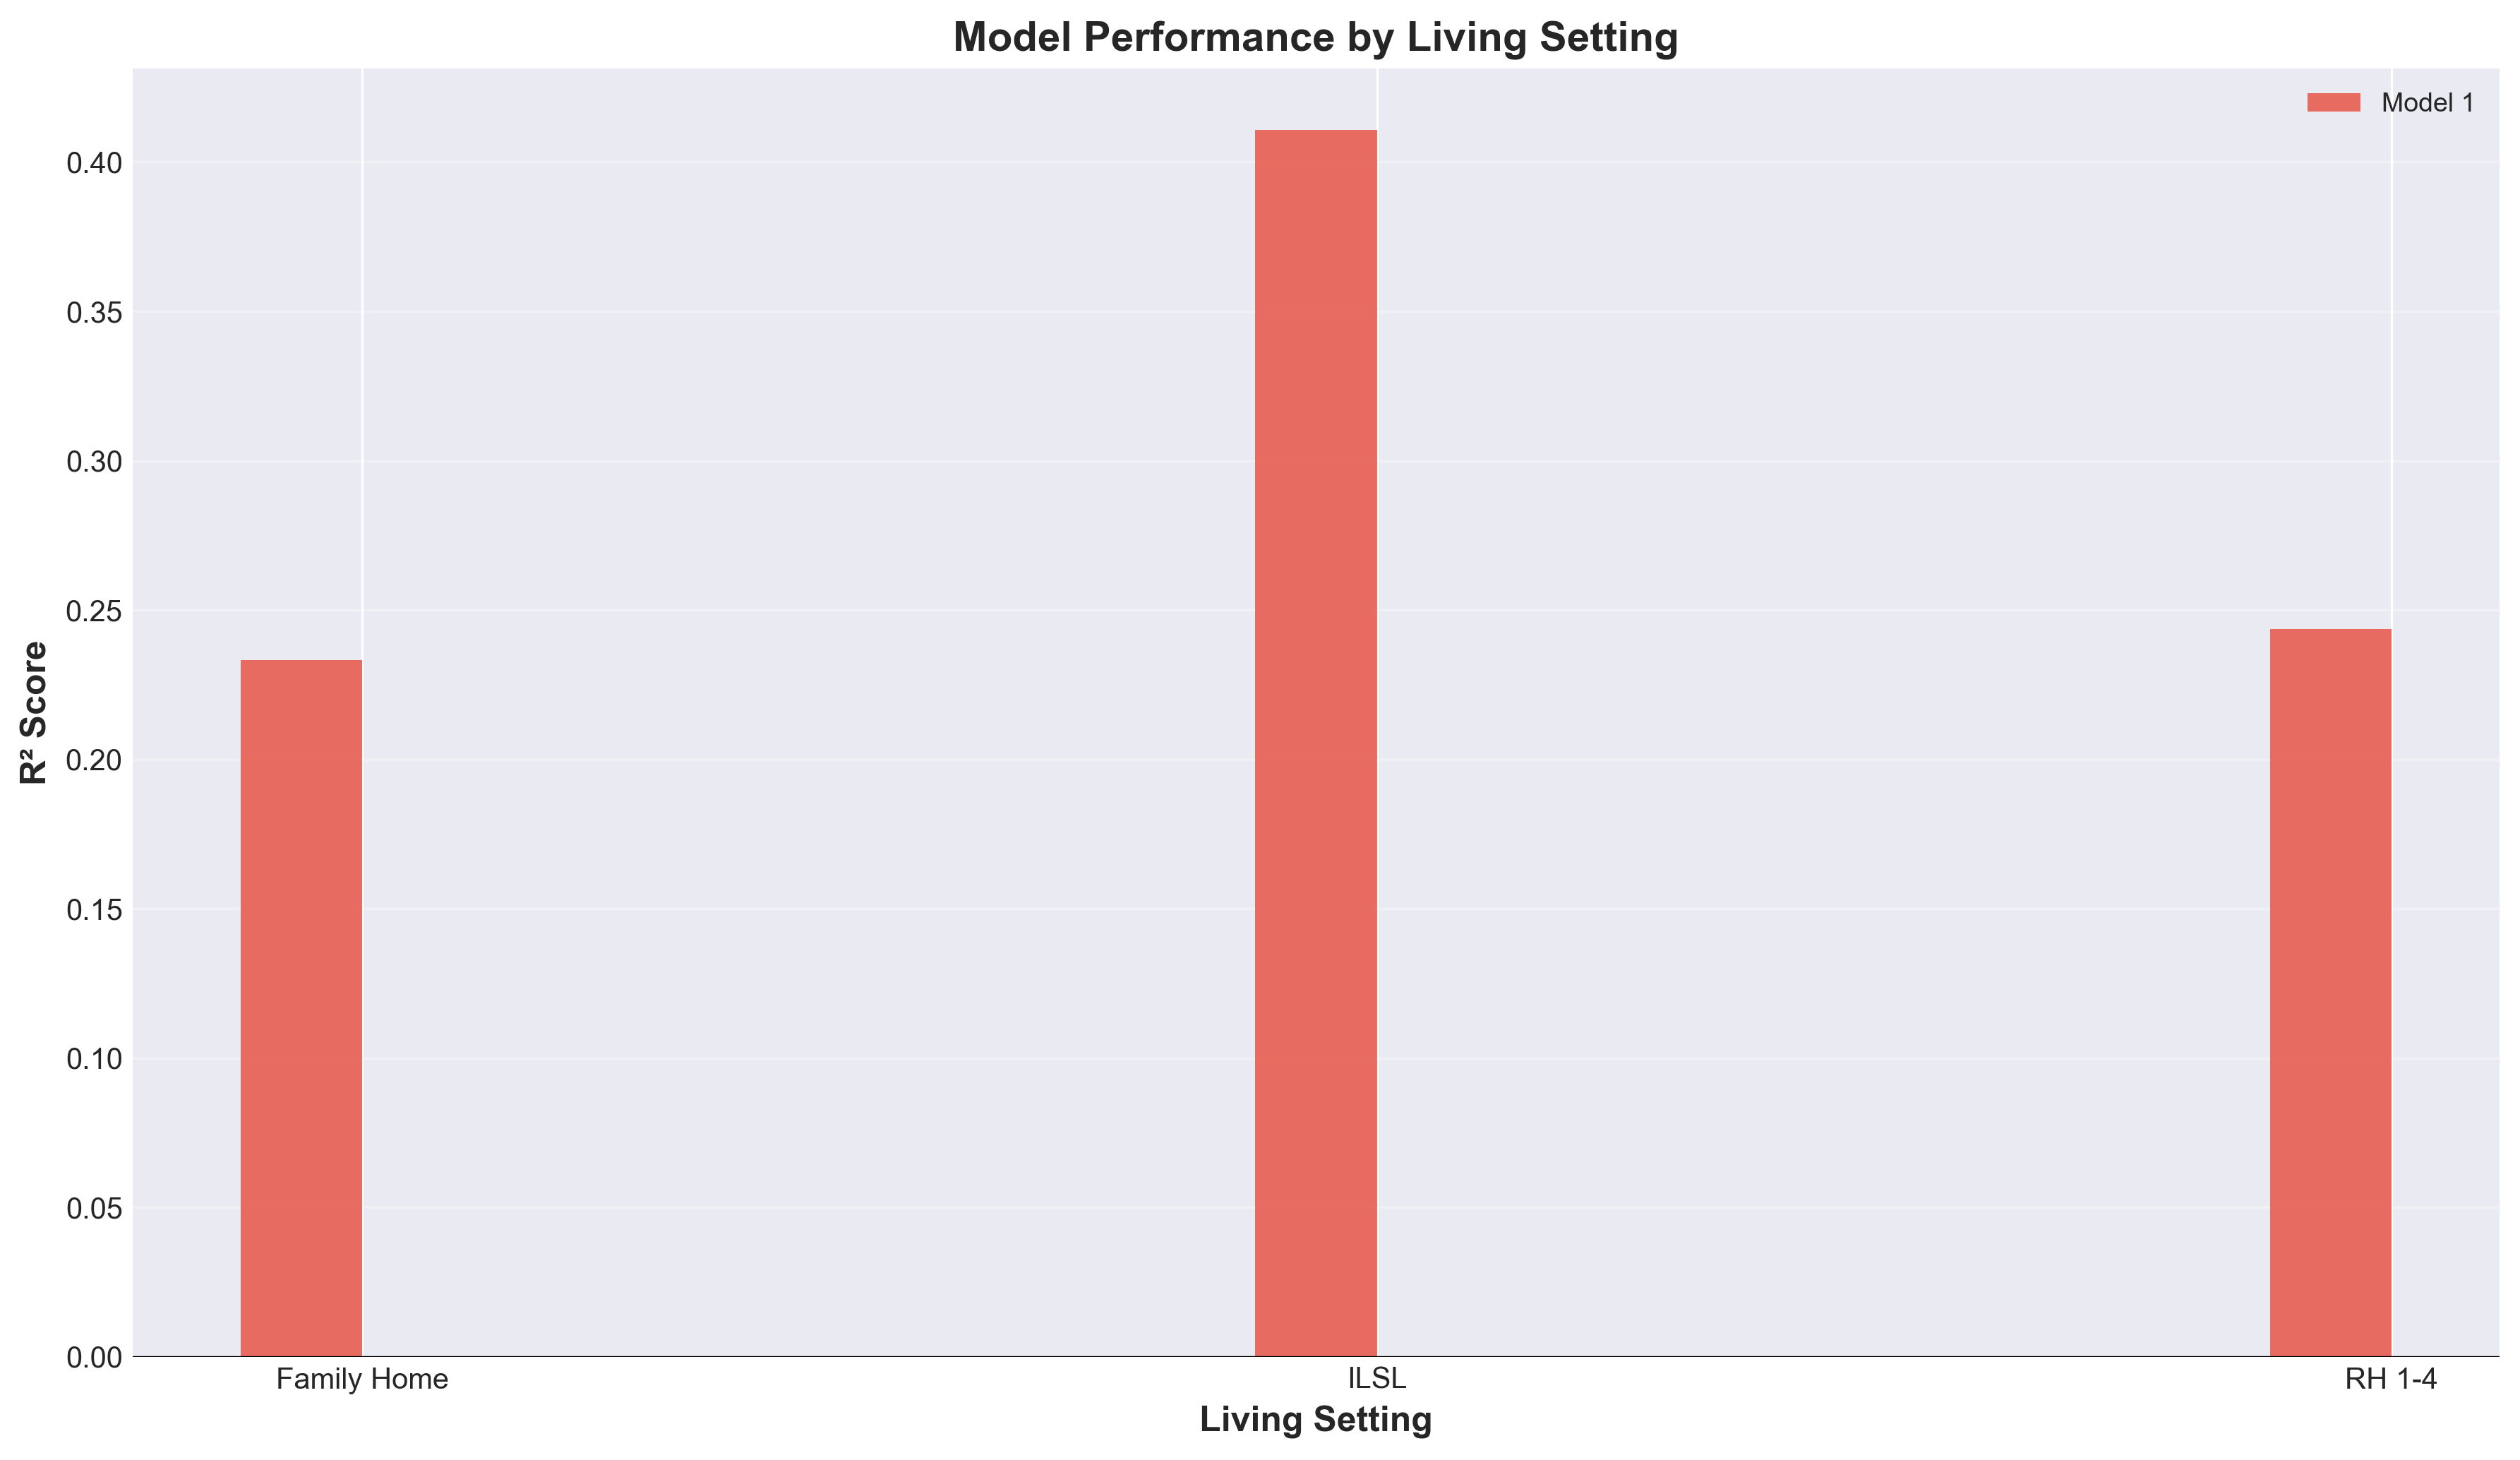
\includegraphics[width=0.95\textwidth]{figures/plot_h_living_setting.png}
\caption{Model Performance by Living Setting}
\label{fig:living_setting_performance}
\end{figure}

Figure \ref{fig:living_setting_performance} compares model performance across the three primary living settings. \textbf{How to interpret}: Taller bars indicate better R² performance for that subgroup. Consistent bar heights across settings suggest a model performs equally well for all living arrangements, while varying heights reveal differential performance. Stakeholders supporting specific populations can identify which models best serve their target groups. Note that negative R² values indicate performance worse than a simple mean prediction.

\begin{figure}[h!]
\centering
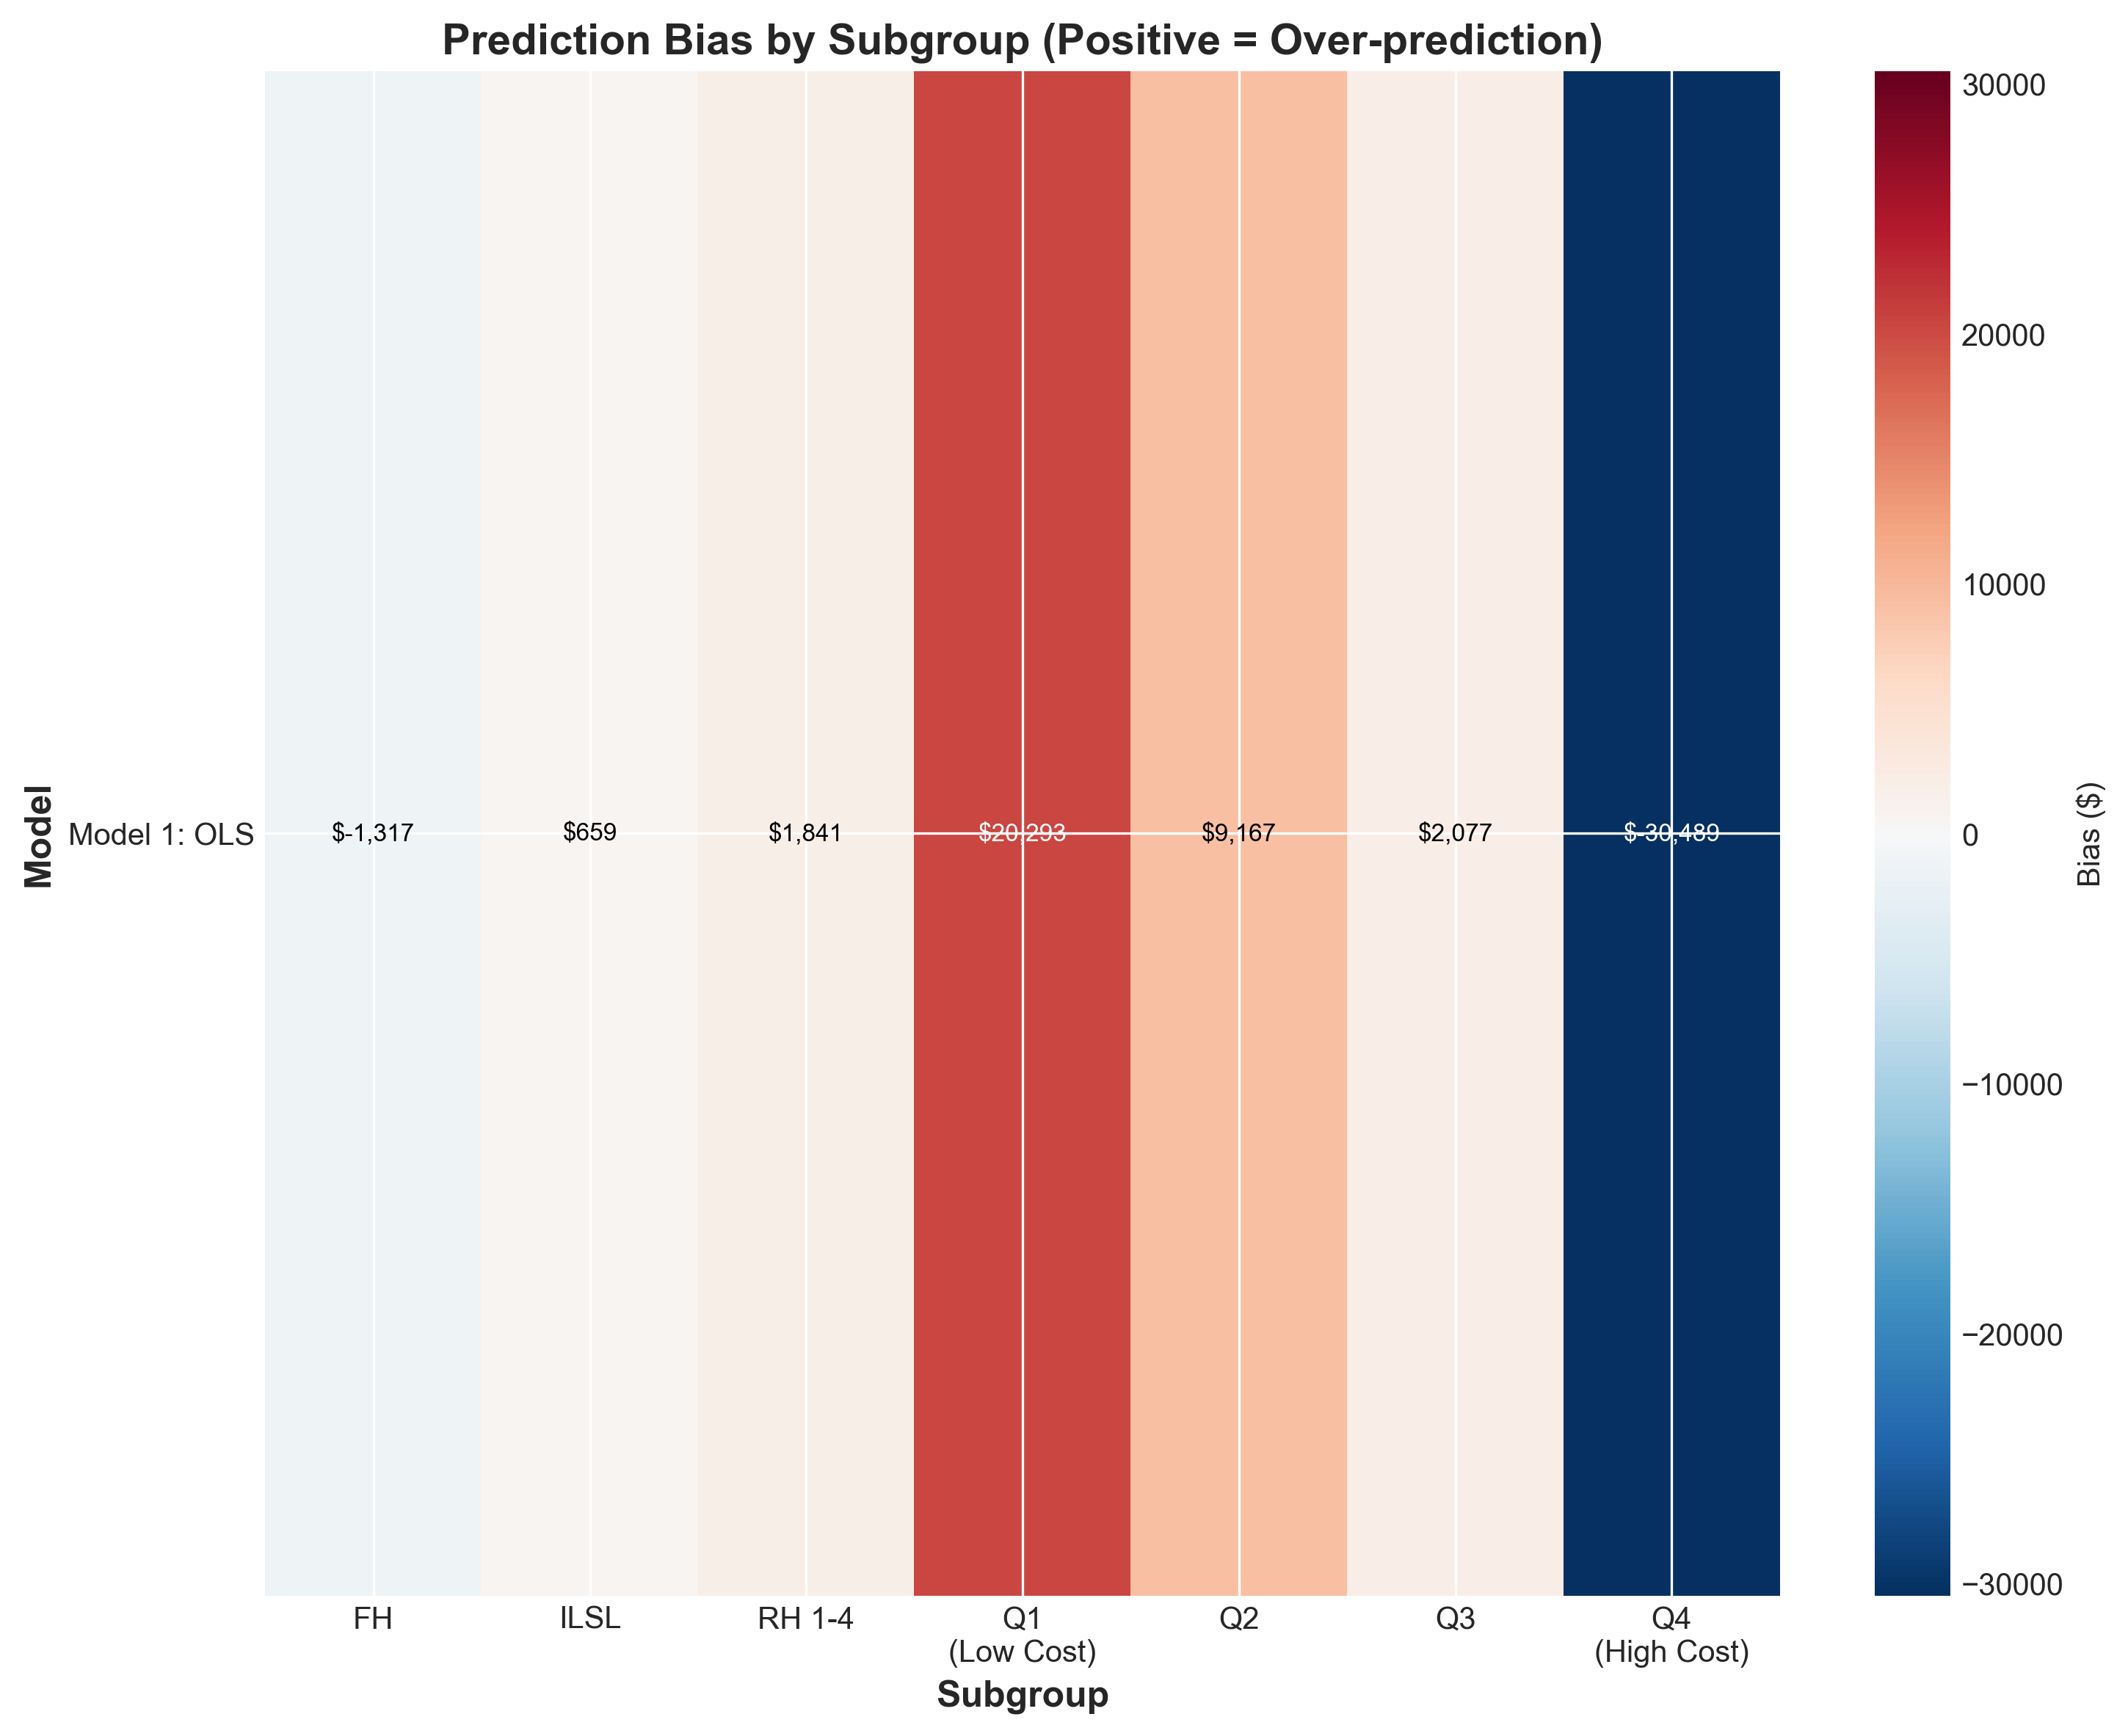
\includegraphics[width=0.85\textwidth]{figures/plot_i_bias_heatmap.png}
\caption{Prediction Bias by Subgroup}
\label{fig:bias_heatmap}
\end{figure}

Figure \ref{fig:bias_heatmap} reveals systematic over- or under-prediction patterns across subgroups. \textbf{How to interpret}: Red cells indicate over-prediction (model predicts higher costs than actual), blue cells indicate under-prediction. Color intensity shows bias magnitude. White (near-zero bias) is ideal, indicating unbiased predictions. This visualization is essential for equity analysis: systematic under-prediction for certain groups could result in inadequate service funding, while over-prediction may indicate inefficient resource allocation. Cost quartile patterns are particularly informative—models often struggle with extreme cases (Q1 and Q4).

\subsection{Interpretation Guidelines for Stakeholders}

\textbf{For Model Selection:}
\begin{itemize}
    \item \textbf{If maximizing explained variance is paramount}: Choose the model with highest R² in Figure \ref{fig:r2_comparison}
    \item \textbf{If minimizing dollar prediction error}: Use Figure \ref{fig:error_metrics} to identify models with lowest RMSE/MAE
    \item \textbf{If operational accuracy targets exist}: Use Figure \ref{fig:cumulative_accuracy} to find models meeting specific tolerance requirements
    \item \textbf{If serving specific populations}: Examine Figures \ref{fig:living_setting_performance} and \ref{fig:bias_heatmap} for subgroup performance
    \item \textbf{If consistency is critical}: Prioritize models with narrow boxes in Figure \ref{fig:cv_stability}
\end{itemize}

\textbf{For Understanding Trade-offs:}
\begin{itemize}
    \item High R² with high RMSE may indicate a model captures variance but makes large errors on difficult cases
    \item Strong overall performance with poor subgroup performance reveals potential equity concerns
    \item Similar training and test performance (Figure \ref{fig:r2_comparison}) indicates good generalization
    \item Divergent RMSE and MAE rankings suggest different error distributions (RMSE more sensitive to outliers)
\end{itemize}